\section{目的}

依講義 PDF 第 111--114 頁重建圖 27.1(a)--(d)，觀察兩相 clock skew、固定輸入與輸出毛刺，檢查 NORA 的邏輯 race 條件與類比完整性之差異。

\section{講義要求與對應測試}

\begin{center}
\small
\setlength{\tabcolsep}{4pt}
\begin{tabular}{p{.42\linewidth}p{.29\linewidth}p{.18\linewidth}}
\toprule
要求 & 網表編號與條件 & 狀態 \\
\midrule
步驟：四電路無 skew 與有 skew & 01; 0, +0.5, -0.5 ns & 各自完整電路 \\
問題 1：輸入固定 0 與 1 & 01; each skew repeated & 9 cases total \\
問題 2：b/c/d 安全性比較 & Settled samples + full waveform & 量測毛刺並討論 \\
\bottomrule
\end{tabular}
\end{center}

\section{拓樸與 NORA 條件}

四組各自使用第一級 clocked inverter、static inverter 及 N-dynamic NAND（另一輸入固定為 1）。(a) 在 N-dynamic 與最後 latch 間放一個 static inverter；(b) 接 P-dynamic 再接 clocked inverter；(c) 接兩個 clocked inverter；(d) 接 clocked inverter 再接 static inverter。每組前級為獨立副本，避免共用節點造成不對等扇出。

NORA 的安全串接要求配合評估方向與反相奇偶：在指定相位區段中，動態與靜態級的反相數及 latch 關係必須符合講義規則，避免 precharge 的非資料轉換穿透到下一個儲存點。但這是邏輯 race 條件，沒有自動消除 charge sharing、clock feedthrough 或有限斜率造成的類比毛刺。

\section{模擬設定與判讀方式}

以提供的加密 MOS 模型、1.0 V 供應、25\,$^\circ$C 為基準。1.0 V 是教學測試條件，並非已核實的額定電壓；沒有把本次結果當作講義原製程或原供應電壓的重現。除網表另註，$W_n/W_p/L=0.6/1.8/0.25\,\mu\mathrm m$，Bulk 接對應電源軌，輸出負載為 5 fF。傳輸閘與弱回授器件的例外尺寸均在網表明列。

使用 PrimeSim HSPICE S-2021.09 win64、\texttt{RUNLVL=6}、\texttt{ACCURATE} 及 \texttt{WARNLIMIT=100}。每份網表的主分析與 \texttt{.alter} 均完成，沒有 error 或 failed measurement；但模擬器仍回報加密區塊的警告被隱藏，因此不能宣稱模型無警告或警告無害。\texttt{.tran} 的列印間隔不是固定積分步長；求解器使用自適應步長。本次沒有把有限的掃描範圍當作完整製程認證。

除非另註，功能診斷以低電位 $V\leq0.2$ V、高電位 $V\geq0.8$ V 判定；這是本報告公開採用的判讀規則，不是講義給定的數值門檻，也不是已萃取的接收器雜訊容限。取樣正確不能排除取樣間毛刺。所有圖均由實際輸出資料重繪；\texttt{results/} 保存逐案例波形、量測與衍生比較 CSV。

公開網表不含模型載入路徑；模擬時在本機副本加入模型設定，模型本體不在交付資料內。網表檔名的前兩位數對應下表編號，各檔可獨立執行。

\section{結果}

週期 4 ns、兩相來源 rise/fall 0.2 ns，互補相位獨立平移 0、+0.5、-0.5 ns。動態輸入與固定 0/1 各重做三種 skew，共 9 分析。每組於 10.6、14.6、18.6、22.6、26.6、30.6 ns 的 6 個穩態樣本均符合反相後資料；但完整波形呈現明顯錯誤脈衝。

\begin{figure}[htbp]
\centering
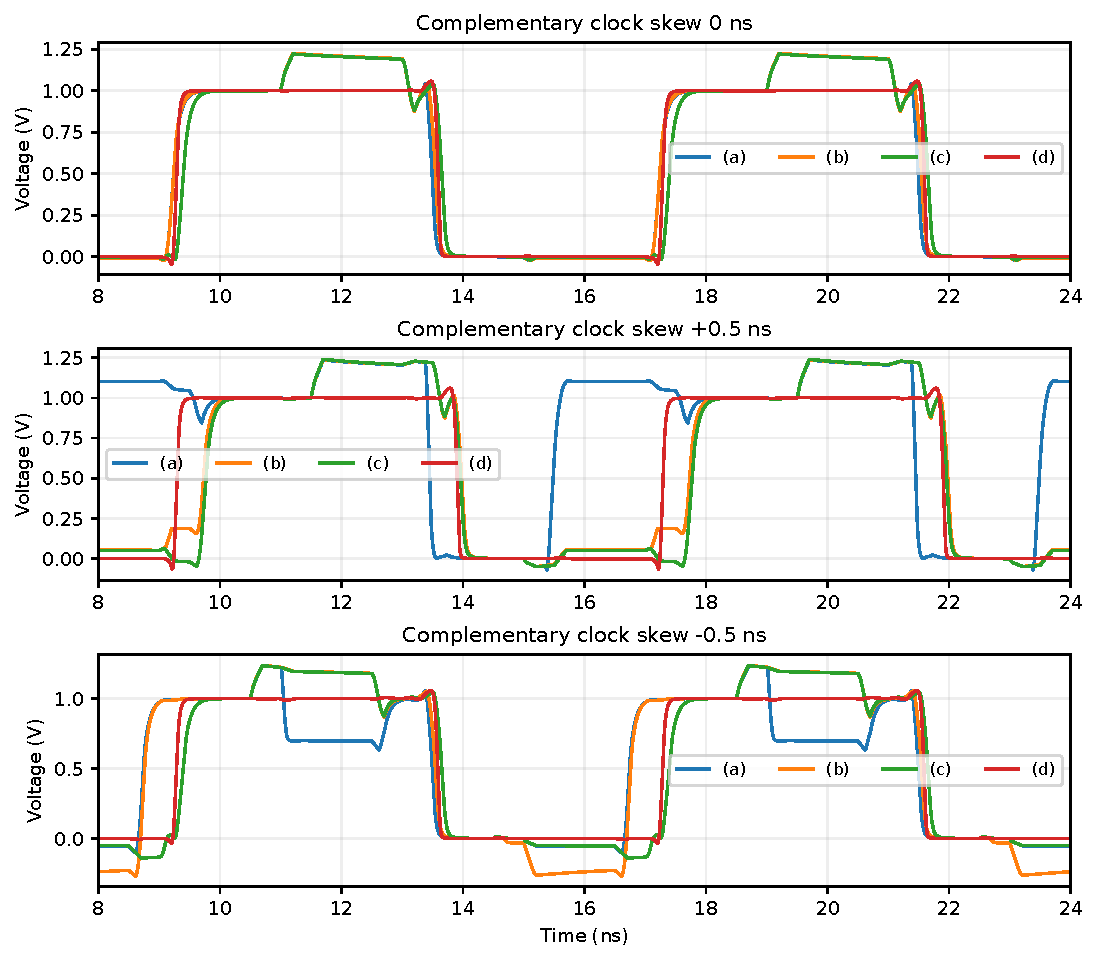
\includegraphics[width=.96\linewidth]{figures/four_topologies.pdf}
\caption{動態資料下的四拓樸；固定時間取樣沒有涵蓋整個保持窗。}
\end{figure}

\begin{center}
\small
\setlength{\tabcolsep}{4pt}
\begin{tabular}{lrrrr}
\toprule
skew (ns) & (a) 最大 (V) & (b) 最大 (V) & (c) 最大 (V) & (d) 最大 (V) \\
\midrule
0 & 0.92728 & 0.95661 & 0.11694 & 0.42357 \\
0.5 & 1.10902 & 0.86663 & 0.14575 & 0.97954 \\
-0.5 & 1.05679 & 1.04569 & 0.17798 & 0.51725 \\
\bottomrule
\end{tabular}
\end{center}

\begin{figure}[htbp]
\centering
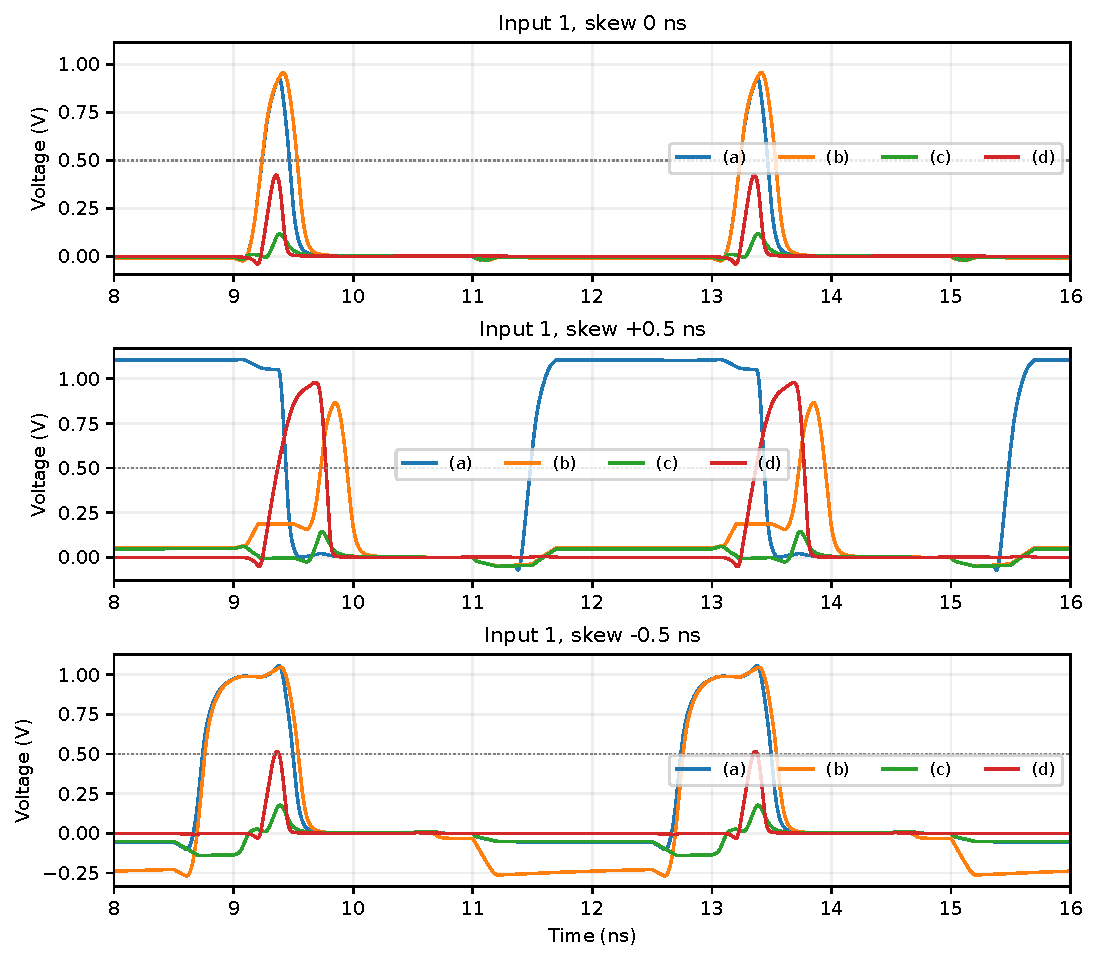
\includegraphics[width=.96\linewidth]{figures/fixed_input_glitches.pdf}
\caption{固定輸入 1，理想輸出應為 0；虛線為 0.5 V 觀察線。}
\end{figure}

固定輸入 1 時，(a) 的錯誤不只出現在資料改變附近，正 skew 下甚至延長為較寬的錯誤高電位。(b) 也有越過 0.5 V 的脈衝；(d) 在 +0.5 ns 時達 0.97954 V。(c) 三種 skew 的峰值最高 0.17798 V，於這組測試最能維持低電位。輸入固定 0 時，(a)/(b)/(c) 的最低值約 0.87 V、最高有約 1.22--1.24 V feedthrough；(d) 高電位更接近電源軌。

\section{討論、差異與尚未證實的範圍}

問題 1 的固定輸入測試排除了「只有資料切換才出現」的解釋；時脈本身的預充、耦合與透明窗即可造成錯誤。問題 2：本組條件下 (c) 低電位保持最穩，但不能由單一模型、負載與三種 skew 宣稱無條件安全。(b)/(d) 的毛刺不能僅憑輸出波形全部歸因為邏輯 race；動態節點電荷與後級放大也會造成同樣外觀。保留內部節點 CSV 供機制追蹤，沒有把 6/6 穩態取樣誤當成整段 race-free 驗收。若設計要求全保持窗不得跨接收器門檻，(a)/(b)/(d) 在本測試尚未滿足；本實驗保留講義拓樸以呈現該差異。
